\documentclass[border=8pt]{standalone}
\usepackage[T1]{fontenc}
\usepackage{libertine}
\usepackage[libertine]{newtxmath}
\usepackage{tikz}
\usetikzlibrary{arrows.meta, positioning, decorations.pathreplacing, calc}

\begin{document}
\begin{tikzpicture}[
    node distance=3.2cm,
    sembox/.style={
      rectangle, rounded corners=3pt, draw, thick,
      minimum height=1.5cm, minimum width=2.4cm,
      font=\small\strut, align=center
    },
    proofdevice/.style={
      sembox, draw=black!40, dashed, fill=white
    },
    arr/.style={-{Stealth[length=5pt]}, thick},
    lbl/.style={font=\scriptsize, align=center, fill=white, inner sep=1pt},
    loc/.style={font=\tiny\itshape, text=black!45},
    dirloc/.style={font=\tiny\itshape, text=black!45, fill=white, inner sep=0pt},
  ]

  % Nodes (single row). The "Concrete" semantics appears in two representations
  % linked by a machine-checked bridge: locally-nameless (de Bruijn, connected to
  % B&P) and named (connected to the timestamped/abstract chain).
  \node[sembox] (bp)   {B\&P\\[-1pt]{\footnotesize (substitution)}\\[-1pt]$\Downarrow_{\mathit{bp}}$};
  \node[sembox, right=of bp] (concln) {Concrete (LN)\\[-1pt]{\footnotesize (de Bruijn)}\\[-1pt]$\Downarrow_{\mathit{eval}}$};
  \node[sembox, right=of concln] (concn) {Concrete (named)\\[-1pt]{\footnotesize (env/store)}\\[-1pt]$\Downarrow_{\mathit{eval}}$};
  \node[proofdevice, right=of concn] (fresh) {Fresh-Guarded\\[-1pt]{\footnotesize (proof device)}\\[-1pt]$\Downarrow^{\kappa\tau f}_{\mathit{eval}}$};
  \node[sembox, right=of fresh] (ts) {Timestamped\\[-1pt]{\footnotesize (paper)}\\[-1pt]$\Downarrow^{\kappa\tau}_{\mathit{eval}}$};
  \node[sembox, right=of ts] (abs) {Abstract\\[-1pt]{\footnotesize (finite)}\\[-1pt]$\widehat{\Downarrow^{\kappa\tau}_{\mathit{eval}}}$};

  % B&P <-> Concrete (LN): the locally-nameless concrete equivalence
  \draw[arr] ([yshift= 3pt] bp.east) -- ([yshift= 3pt] concln.west)
    node[lbl, midway, above=2pt] {Completeness};
  \draw[arr] ([yshift=-3pt] concln.west) -- ([yshift=-3pt] bp.east)
    node[lbl, midway, below=2pt] {Soundness};
  \node[dirloc, above] at ($(bp)!0.5!(concln) + (0,0.55)$) {${\sim}0.7$k\,\textnormal{+}\,$0.6$k loc};
  \node[loc] at ($(bp)!0.5!(concln) + (0,-0.95)$) {locally nameless};
  \node[loc] at ($(bp)!0.5!(concln) + (0,-1.25)$) {+ ${\sim}1.2$k shared};

  % Concrete (LN) <-> Concrete (named): the bridge (bidirectional simulation)
  \draw[arr] ([yshift= 3pt] concln.east) -- ([yshift= 3pt] concn.west)
    node[lbl, midway, above=2pt] {Completeness};
  \draw[arr] ([yshift=-3pt] concn.west) -- ([yshift=-3pt] concln.east)
    node[lbl, midway, below=2pt] {Soundness};
  \node[dirloc, above] at ($(concln)!0.5!(concn) + (0,0.55)$) {Bridge};
  \node[loc] at ($(concln)!0.5!(concn) + (0,-0.95)$) {${\sim}1.5$k loc};
  \node[loc] at ($(concln)!0.5!(concn) + (0,-1.25)$) {(well-formed progs)};

  % Concrete (named) <-> Fresh-Guarded
  \draw[arr] ([yshift= 3pt] concn.east) -- ([yshift= 3pt] fresh.west)
    node[lbl, midway, above=2pt] {Completeness};
  \draw[arr] ([yshift=-3pt] fresh.west) -- ([yshift=-3pt] concn.east)
    node[lbl, midway, below=2pt] {Soundness};
  \node[dirloc, above] at ($(concn)!0.5!(fresh) + (0,0.55)$) {${\sim}3.9$k\,\textnormal{+}\,$1.2$k loc};
  \node[loc] at ($(concn)!0.5!(fresh) + (0,-1.1)$) {+ ${\sim}0.5$k shared};

  % Fresh-Guarded <-> Timestamped
  \draw[arr] ([yshift= 3pt] fresh.east) -- ([yshift= 3pt] ts.west)
    node[lbl, midway, above=2pt] {Completeness};
  \draw[arr] ([yshift=-3pt] ts.west) -- ([yshift=-3pt] fresh.east)
    node[lbl, midway, below=2pt] {Soundness (freshness)};
  \node[dirloc, above] at ($(fresh)!0.5!(ts) + (0,0.55)$) {${\sim}0.1$k\,\textnormal{+}\,$2.4$k loc};
  \node[loc] at ($(fresh)!0.5!(ts) + (0,-1.1)$) {+ ${\sim}3.2$k shared};

  % Timestamped -> Abstract (one direction only)
  \draw[arr] (ts.east) -- (abs.west)
    node[lbl, midway, below=2pt] {Soundness};
  \node[dirloc, above] at ($(ts)!0.5!(abs) + (0,0.55)$) {${\sim}0.6$k loc};

  % Component line counts below boxes
  \node[loc] at ($(bp) + (0,-1.1)$) {${\sim}0.8$k loc};
  \node[loc] at ($(concln) + (0,-1.1)$) {${\sim}0.7$k loc};
  \node[loc] at ($(concn) + (0,-1.1)$) {${\sim}0.8$k loc};
  \node[loc] at ($(fresh) + (0,-1.1)$) {${\sim}0.8$k loc};
  \node[loc] at ($(ts) + (0,-1.1)$) {${\sim}0.4$k loc};
  \node[loc] at ($(abs) + (0,-1.1)$) {${\sim}0.3$k loc};

  % Grand total
  \node[font=\footnotesize, text=black!55] at ($(concn)!0.5!(fresh) + (0,-1.9)$)
    {${\sim}3.2$k definitions\enspace$+$\enspace${\sim}16.9$k proofs\enspace$=$\enspace${\sim}20$k Lean 4};

\end{tikzpicture}
\end{document}
